% Editable vector schematic; input tokens illustrate visibility, not measured data.
\documentclass[tikz,border=0pt]{standalone}
\usepackage{fontspec}
\setsansfont{LiberationSans}[Path=../../shared/assets/,Extension=.ttf,UprightFont=*-Regular,BoldFont=*-Bold]
\usepackage{amsmath}
\usetikzlibrary{arrows.meta,calc}
\definecolor{ink}{HTML}{0C0C0C}
\definecolor{muted}{HTML}{63676B}
\definecolor{learn}{HTML}{007C83}
\definecolor{copycolor}{HTML}{A36F23}
\definecolor{teacherfill}{HTML}{FBF5EA}
\definecolor{studentfill}{HTML}{EDF6F5}
\hyphenpenalty=10000\exhyphenpenalty=10000
\begin{document}
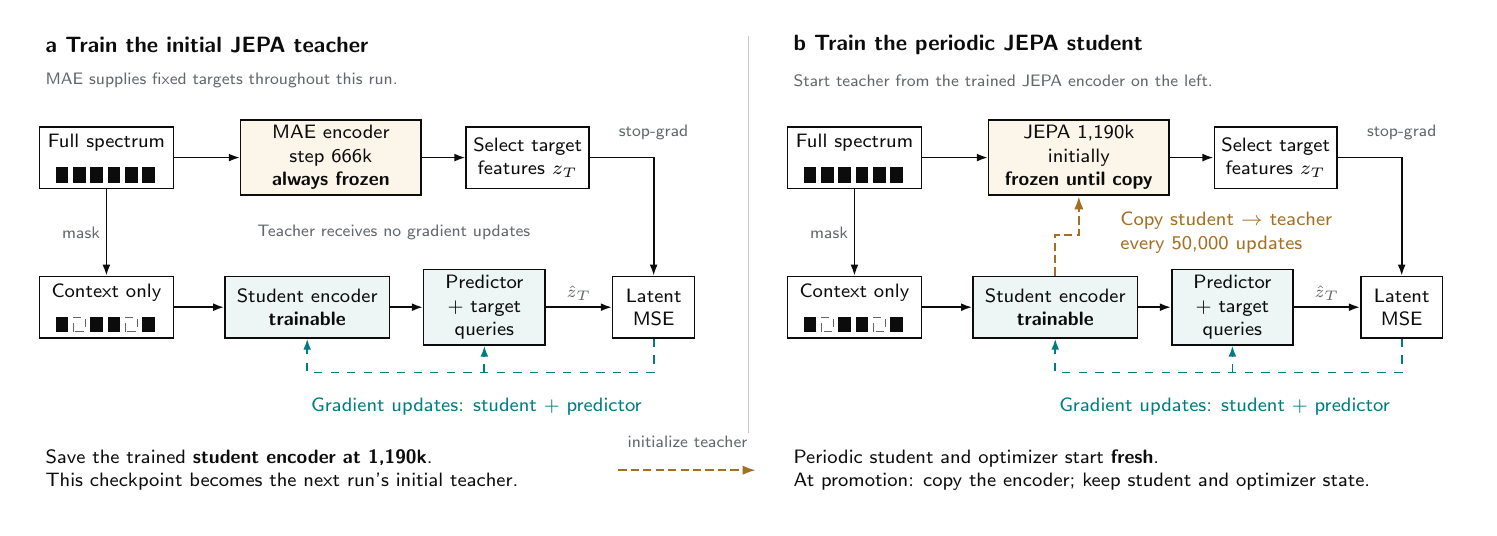
\begin{tikzpicture}[x=1cm,y=1cm,
 every node/.style={font=\sffamily\fontsize{7}{8.5}\selectfont,text=ink,align=center,inner sep=2pt},
 block/.style={draw=ink,line width=.55pt,minimum height=.78cm},
 forward/.style={-{Latex[length=1.4mm,width=1mm]},line width=.65pt,draw=ink},
 gradient/.style={-{Latex[length=1.4mm,width=1mm]},line width=.65pt,draw=learn,dashed},
 copyweight/.style={-{Latex[length=1.7mm,width=1.2mm]},line width=.9pt,draw=copycolor,dash pattern=on 3pt off 1.5pt},
 smallnote/.style={font=\sffamily\fontsize{6.5}{8}\selectfont,text=muted}]
\path[use as bounding box] (0,0) rectangle (18.3,6.1);
\draw[muted!35,line width=.4pt] (9.15,.95)--(9.15,6.0);
\foreach \offset/\stage in {0/0,9.5/1}{
 \begin{scope}[shift={(\offset,0)}]
  \ifnum\stage=0
   \node[anchor=west,font=\sffamily\bfseries\fontsize{8}{10}\selectfont] at (.15,5.88) {a  Train the initial JEPA teacher};
   \node[anchor=west,smallnote] at (.15,5.43) {MAE supplies fixed targets throughout this run.};
   \node[block,fill=teacherfill,text width=2.15cm] (teacher) at (3.85,4.45) {MAE encoder\\step 666k\\\textbf{always frozen}};
  \else
   \node[anchor=west,font=\sffamily\bfseries\fontsize{8}{10}\selectfont] at (.15,5.88) {b  Train the periodic JEPA student};
   \node[anchor=west,smallnote] at (.15,5.43) {Start teacher from the trained JEPA encoder on the left.};
   \node[block,fill=teacherfill,text width=2.15cm] (teacher) at (3.85,4.45) {JEPA 1,190k initially\\\textbf{frozen until copy}};
  \fi
  \node[block,minimum width=1.7cm,minimum height=.78cm] (full) at (1.0,4.45) {};
  \node at (1.0,4.64) {Full spectrum};
  \node[block,minimum width=1.7cm,minimum height=.78cm] (context) at (1.0,2.55) {};
  \node at (1.0,2.74) {Context only};
  \foreach \i in {0,...,5}{
   \draw[fill=ink,draw=ink,line width=.3pt] ({.36+.22*\i},4.14) rectangle +( .15,.18);
   \ifnum\i=1
    \draw[draw=muted,densely dashed,line width=.3pt] ({.36+.22*\i},2.24) rectangle +(.15,.18);
   \else\ifnum\i=4
    \draw[draw=muted,densely dashed,line width=.3pt] ({.36+.22*\i},2.24) rectangle +(.15,.18);
   \else
    \draw[fill=ink,draw=ink,line width=.3pt] ({.36+.22*\i},2.24) rectangle +(.15,.18);
   \fi\fi
  }
  \node[block,text width=1.42cm] (targets) at (6.35,4.45) {Select target\\features $z_T$};
  \node[block,fill=studentfill,text width=1.95cm] (student) at (3.55,2.55) {Student encoder\\\textbf{trainable}};
  \node[block,fill=studentfill,text width=1.4cm] (predictor) at (5.8,2.55) {Predictor\\+ target queries};
  \node[block,text width=.9cm,minimum height=.78cm] (loss) at (7.95,2.55) {Latent\\MSE};
  \draw[forward] (full.south)--node[left,smallnote] {mask}(context.north);
  \draw[forward] (full.east)--(teacher.west);
  \draw[forward] (teacher.east)--(targets.west);
  \draw[forward] (targets.east)-|(loss.north);
  \node[smallnote] at (7.95,4.77) {stop-grad};
  \draw[forward] (context.east)--(student.west);
  \draw[forward] (student.east)--(predictor.west);
  \draw[forward] (predictor.east)--node[above,smallnote] {$\hat z_T$}(loss.west);
  \draw[gradient] (loss.south)--(7.95,1.72)--(3.55,1.72)--(student.south);
  \draw[gradient] (5.8,1.72)--(predictor.south);
  \node[text=learn] at (5.7,1.29) {Gradient updates: student + predictor};
  \ifnum\stage=0
   \node[smallnote] at (4.65,3.5) {Teacher receives no gradient updates};
  \else
   \draw[copyweight] (student.north)--(3.55,3.47)--(3.85,3.47)--(teacher.south);
   \node[text=copycolor,anchor=west,align=left] at (4.3,3.5) {Copy student $\rightarrow$ teacher\\every 50,000 updates};
  \fi
 \end{scope}
}
\node[anchor=west,align=left] at (.15,.48) {Save the trained \textbf{student encoder at 1,190k}.\\This checkpoint becomes the next run's initial teacher.};
\draw[copyweight] (7.5,.48)--(9.25,.48);
\node[smallnote] at (8.38,.84) {initialize teacher};
\node[anchor=west,align=left] at (9.65,.48) {Periodic student and optimizer start \textbf{fresh}.\\At promotion: copy the encoder; keep student and optimizer state.};
\end{tikzpicture}
\end{document}
